\documentclass[10pt]{beamer}

\usetheme{Boadilla}
\usecolortheme{seahorse}

%\setbeamercovered{transparent}

\setbeamertemplate{section in toc}{$\circ$ \inserttocsection}
\setbeamertemplate{itemize item}{\scriptsize\raise1.25pt\hbox{\donotcoloroutermaths$\blacktriangleright$}}
\setbeamertemplate{itemize subitem}{\tiny\raise1.5pt\hbox{\donotcoloroutermaths$\blacktriangleright$}}
\setbeamertemplate{itemize subsubitem}{\tiny\raise1.5pt\hbox{\donotcoloroutermaths$\blacktriangleright$}}
\setbeamertemplate{enumerate item}{\insertenumlabel.}
\setbeamertemplate{enumerate subitem}{\insertenumlabel.\insertsubenumlabel}
\setbeamertemplate{enumerate subsubitem}{\insertenumlabel.\insertsubenumlabel.\insertsubsubenumlabel}
\setbeamertemplate{enumerate mini template}{\insertenumlabel}

\usepackage[english]{babel}
\usepackage[latin1]{inputenc}
\usepackage{libertine}
\usepackage[T1]{fontenc}

%%
\usepackage{xspace}
\usepackage{msthpres}
\newcommand{\gpucb}{\textsf{GP-UCB}\xspace}
\newcommand{\gpbucb}{\textsf{GP-BUCB}\xspace}
\newcommand{\acl}{\textsf{LSE}\xspace}
\newcommand{\fullacl}{Level Set Estimation\xspace}
\newcommand{\iacl}{\textsf{LSE\textsubscript{imp}}\xspace}
\newcommand{\bacl}{\textsf{LSE\textsubscript{batch}}\xspace}
\newcommand{\ibacl}{\textsf{LSE\textsubscript{imp-batch}}\xspace}
\newcommand{\str}{\textsf{STR}\xspace}
\newcommand{\istr}{\textsf{STR\textsubscript{imp}}\xspace}
\newcommand{\bstr}{\textsf{STR\textsubscript{batch}}\xspace}
\newcommand{\rstr}{\textsf{STR\textsubscript{rank}}\xspace}
\newcommand{\var}{\textsf{VAR}\xspace}
%%


\newcommand{\qauth}[1]{{\footnotesize\par\normalfont\hfill---\ \emph{#1}\par}}

\title[Active Learning for Level Set Estimation]
{Active Learning for Level Set Estimation}

\author[Alkis Gkotovos]{
\footnotesize
M.Sc. Thesis by Alkis Gkotovos\\
Department of Computer Science\\
ETH Zurich
}

\date[M.Sc. Thesis presentation]{
\footnotesize
Supervised by Prof. Andreas Krause

}

%\subject{Theoretical Computer Science}
% This is only inserted into the PDF information catalog. Can be left
% out. 



% If you have a file called "university-logo-filename.xxx", where xxx
% is a graphic format that can be processed by latex or pdflatex,
% resp., then you can add a logo as follows:

%\pgfdeclareimage[height=0.5cm]{university-logo}{figures/eth_logo_black.pdf}
%\logo{\pgfuseimage{university-logo}}


% If you wish to uncover everything in a step-wise fashion, uncomment
% the following command: 
%\beamerdefaultoverlayspecification{<+->}


\begin{document}

\begin{frame}
  \titlepage
\end{frame}

\begin{frame}{Outline}
  \tableofcontents
  % You might wish to add the option [pausesections]
\end{frame}


\section{Motivation and Background}

\begin{frame}
\begin{center}
Swimmers of Lake Zurich, beware!\\
\vspace{0.2in}
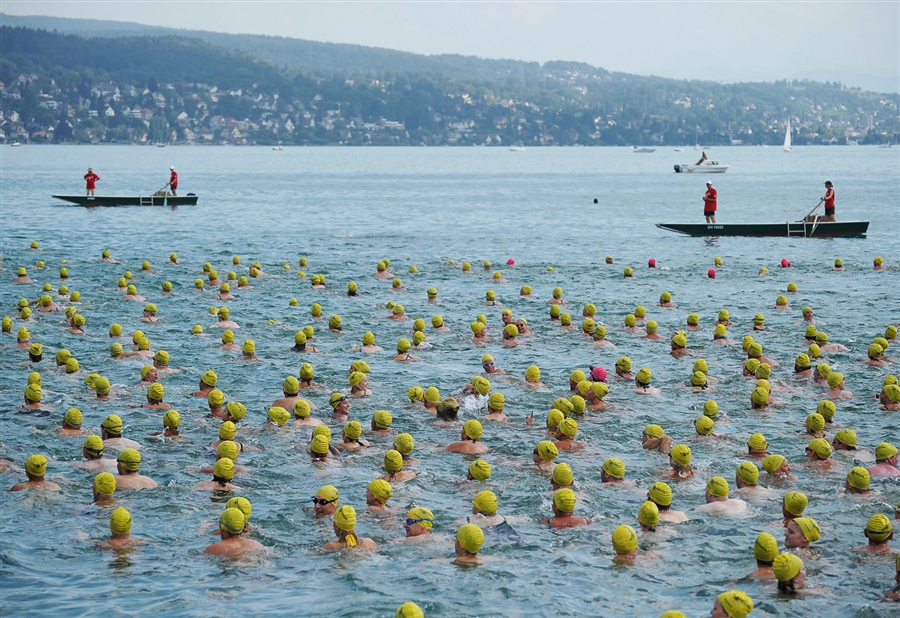
\includegraphics[width=4in]{figures/swimmers.jpg}\\[-0.5em]
{\tiny (Source: Steffen Schmidt / EPA)}
\end{center}
\end{frame}

\begin{frame}
\begin{center}
\uncover<1->{Swimmers of Lake Zurich, beware!}
\vspace{0.2in}
\begin{columns}[c]
\column{0.4\textwidth}
\uncover<1->{
\minipage[c][0.75\textheight][s]{\columnwidth}
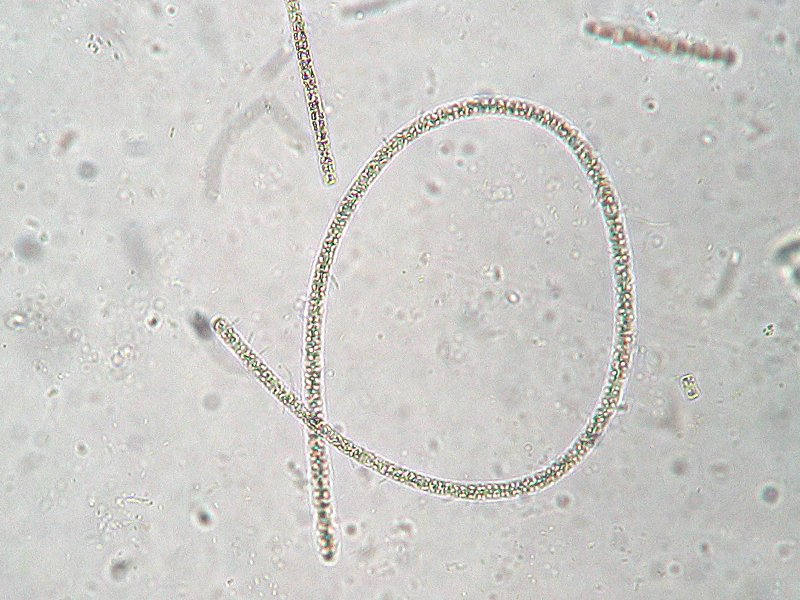
\includegraphics[width=1.7in]{figures/pr.jpeg}\\[-0.5em]
{\tiny (Source: www.limnobotics.ch)}\\
\vfill
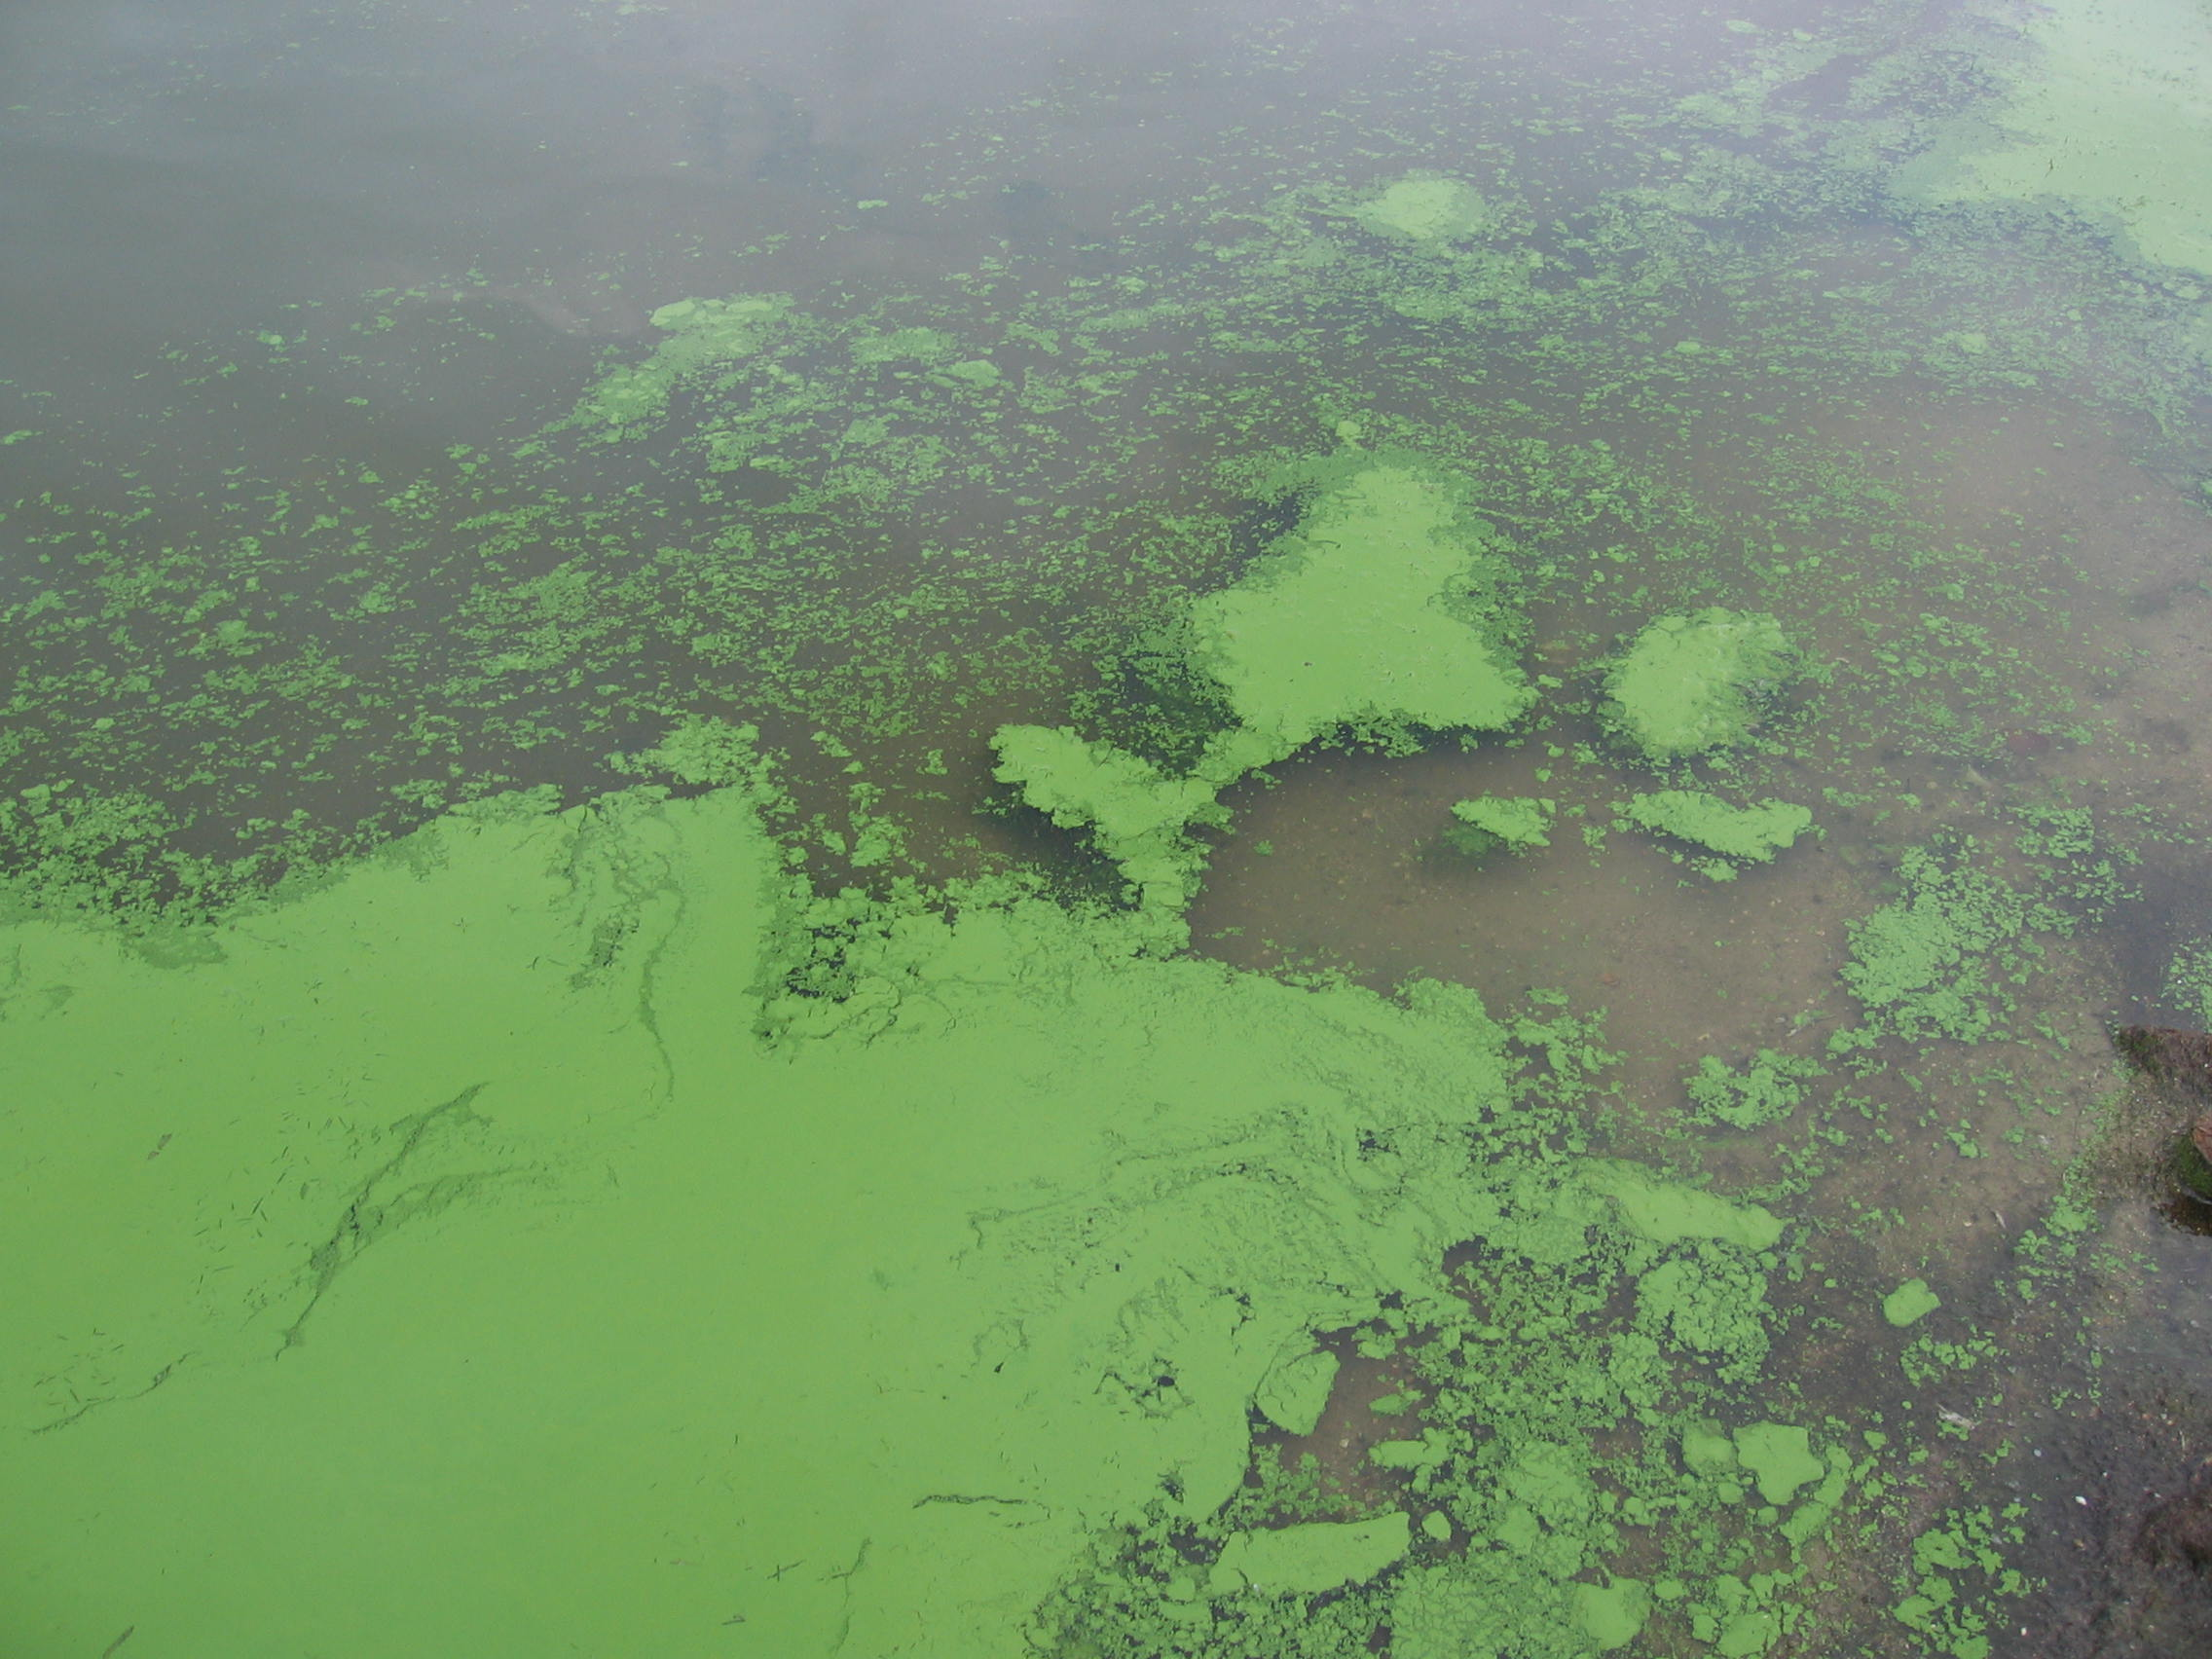
\includegraphics[width=1.7in]{figures/bloom.jpg}\\[-0.5em]
{\tiny (Source: Flickr/Dr. Jennifer L. Graham/U.S. Geological Survey)}
\endminipage
}

\column{0.6\textwidth}
\minipage[c][0.75\textheight][s]{\columnwidth}
\uncover<1->{
\small
``The warming waters of one of central Europe's most popular holiday
destinations, Switzerland's Lake Zurich, have created an ideal environment
for a population explosion of algae including \emph{Planktothrix rubescens},
[...]''
\qauth{Scientific American}
}
\vfill
\uncover<2->{
\small
``\emph{Planktotrhix rubescens} can account for half of the total
phytoplankton biomass in Lake Zurich in summer [...]''
\vspace{1em}

``\emph{Planktotrhix rubescens} are among the most important
producers of hepatotoxic microcystins in freshwaters [...]''
\qauth{Silke Van den Wyngaert \emph{et al.}, ASLO, 2011}
}
\vfill
\uncover<3->{
\small
``Microcystins [...] are cyanotoxins and can be very toxic for plants and
animals including humans.
Their hepatotoxicity may cause serious damage to the liver.''
\qauth{Wikipedia}
}
\endminipage
\end{columns}
\end{center}
\end{frame}

\begin{frame}
\begin{center}
\vspace{0.2in}
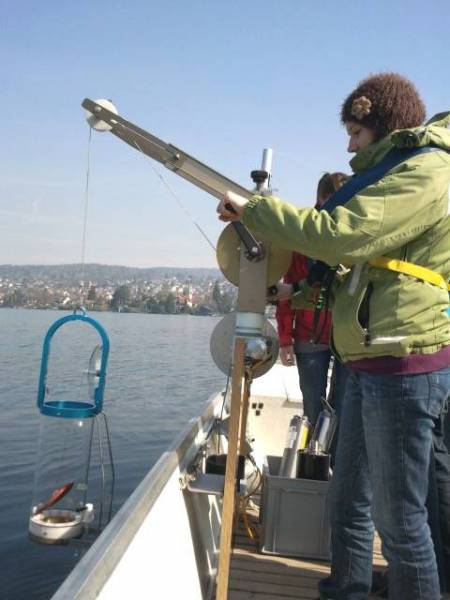
\includegraphics[width=2in]{figures/manual.jpg}\\[-0.5em]
{\tiny (Source: www.limnobotics.ch)}
\end{center}
\end{frame}

\begin{frame}
\begin{center}
\vspace{0.2in}
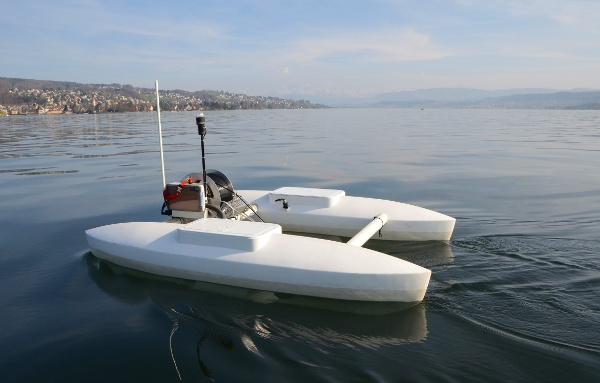
\includegraphics[width=4in]{figures/boat.jpg}\\[-0.5em]
{\tiny (Source: www.limnobotics.ch)}
\end{center}
\end{frame}

\begin{frame}
\begin{center}
\vspace{0.2in}
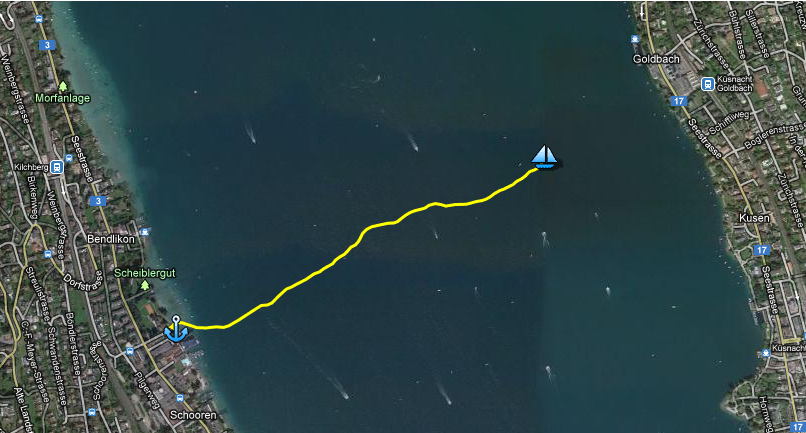
\includegraphics[width=4in]{figures/lake.png}\\[-0.5em]
{\tiny (Source: www.limnobotics.ch)}
\end{center}
\end{frame}

\begin{frame}
\begin{center}
\vspace{0.2in}
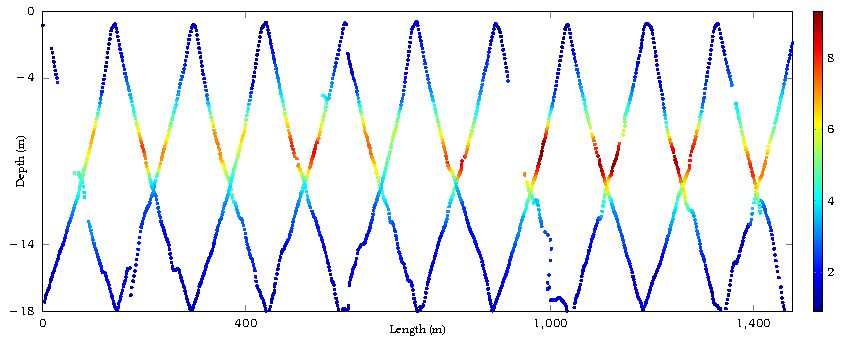
\includegraphics[width=4.7in]{figures/limno_bgape_sc}
\end{center}
\end{frame}

\begin{frame}
\begin{center}
\vspace{0.2in}
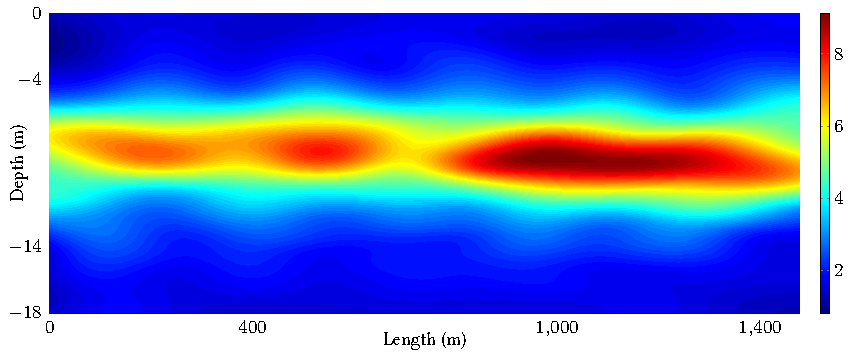
\includegraphics[width=4.7in]{figures/limno_bgape}
\end{center}
\end{frame}

\begin{frame}
\begin{center}
\vspace{0.2in}
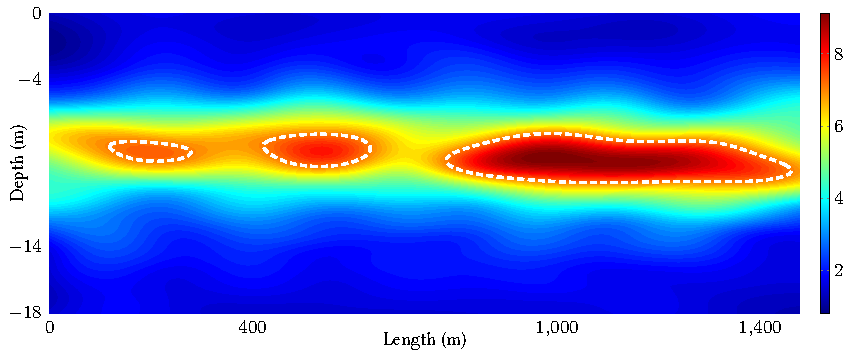
\includegraphics[width=4.7in]{figures/limno_bgape_ls}
\end{center}
\end{frame}

\begin{frame}
\begin{center}
\vspace{0.2in}
\hspace{-2em}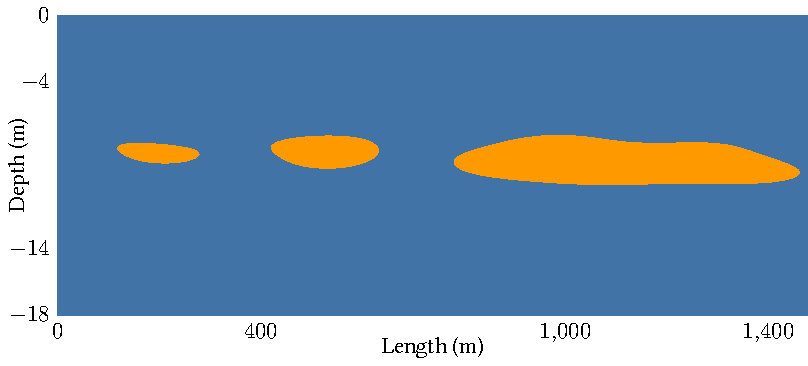
\includegraphics[width=4.45in]{figures/limno_bgape_cl}
\end{center}
\end{frame}

\begin{frame}
\begin{itemize}
\item<1-> Pose as a sequential decision making problem (\emph{pool-based active learning}):
\begin{itemize}
\item<2-> No measurements available in advance, just a set (pool) of possible sampling locations ($D$)
\vspace{0.5em}
\item<3->[]\hspace{-1.5em} At each iteration $t \geq 1$:
\item<3-> Decide where to measure next ($x_t$)
\item<4-> Obtain noisy observation ($y_t = f(x_t) + n_t$)
\item<5-> Update our estimate of the underlying function (e.g. algae concentration)
\end{itemize}
\end{itemize}
\begin{center}
\color{white}
\includegraphics<1>[draft,width=4.45in]{figures/oned_0}
\color{black}
\includegraphics<2>[width=4.45in]{figures/oned_0}
\includegraphics<3>[width=4.45in]{figures/oned_1_0}
\includegraphics<4>[width=4.45in]{figures/oned_1_1}
\includegraphics<5>[width=4.45in]{figures/oned_1_2}
\includegraphics<6>[width=4.45in]{figures/oned_2_0}
\includegraphics<7>[width=4.45in]{figures/oned_2_1}
\includegraphics<8>[width=4.45in]{figures/oned_2_2}
\end{center}
\end{frame}

\begin{frame}
\begin{enumerate}
\item<1-> How do we \textbf{estimate} the function?
\vspace{1em}
\item<2-> How do we \textbf{classify}?
\vspace{1em}
\item<3-> Each measurement is expensive (time, battery power).\\
      How do we \textbf{select} ``informative'' measurements?
\end{enumerate}
\vspace{2em}
\begin{center}
\uncover<4->{\large
Gaussian processes to the rescue!
}
\end{center}
\end{frame}

\begin{frame}
\begin{center}
\uncover<1->{\large Why GPs are nice}
\end{center}
\begin{itemize}
\item<2-> \textbf{Nonparametric}:\\
      Impose ``smoothness'' assumptions via kernel $k(x, x')$.
\vspace{1em}
\item<3-> \textbf{Bayesian}, yet \textbf{efficient}:
      \begin{align*}
        \mu_t(\*x) &= \*k_t(\*x)^T\left(\*K_t + \sigma^2 \*I\right)^{-1}\*y_t\\
        k_t(\*x, \*x') &= k(\*x, \*x') - \*k_t(\*x)^T\left(\*K_t + \sigma^2 \*I\right)^{-1}\*k_t(\*x)\notag\\
        \sigma_t^2(\*x) &= k_t(\*x, \*x)
      \end{align*}
      Suitable for step-by-step updates.
\vspace{1em}
\item<4-> More importantly: they provide \textbf{variance estimates}!\\
          Construct confidence intervals: $Q_t(\*x) = \left[\mu_{t-1}(\*x) \pm \beta_t \sigma_{t-1}(\*x)\right]$
\end{itemize}
\end{frame}

\begin{frame}
\begin{center}
\includegraphics<1>[width=4.45in]{figures/voned_0}
\includegraphics<2>[width=4.45in]{figures/voned_1_0}
\includegraphics<3>[width=4.45in]{figures/voned_1_1}
\includegraphics<4>[width=4.45in]{figures/voned_1_2}
\includegraphics<5>[width=4.45in]{figures/voned_2_0}
\includegraphics<6>[width=4.45in]{figures/voned_2_1}
\includegraphics<7>[width=4.45in]{figures/voned_2_2}
\includegraphics<8>[width=4.45in]{figures/voned_3_0}
\includegraphics<9>[width=4.45in]{figures/voned_3_1}
\includegraphics<10>[width=4.45in]{figures/voned_3_2}
\end{center}
\end{frame}

\begin{frame}
\begin{enumerate}
\item<1-> How do we \textbf{estimate} the function? \uncover<3->{\Large\color{green!70!black}\checkmark}
\vspace{0em}
\item<4-> How do we \textbf{classify}? \uncover<14->{\Large\color{green!70!black}\checkmark}
\vspace{0.3em}
\item<15-> How do we \textbf{select} ``informative'' measurements? \uncover<24->{\Large\color{green!70!black}\checkmark}
\uncover<16->{
\begin{itemize}
\item<16-> Pick among the yet unclassified.
\item<17-> Doesn't really matter which!\\
           \uncover<18->{(e.g. max. variance, }\uncover<19->{max. ambiguity}\uncover<23->{, or even random)}
\end{itemize}}
\end{enumerate}

\begin{center}
\color{white}
\includegraphics<1>[draft,width=3.5in]{figures/voned_cl_00}
\color{black}
\includegraphics<2-4>[width=3.5in]{figures/voned_cl_00}
\includegraphics<5>[width=3.5in]{figures/voned_cl_01}
\includegraphics<6>[width=3.5in]{figures/voned_cl_10}
\includegraphics<7>[width=3.5in]{figures/voned_cl_11}
\includegraphics<8>[width=3.5in]{figures/voned_cl_20}
\includegraphics<9>[width=3.5in]{figures/voned_cl_21}
\includegraphics<10>[width=3.5in]{figures/voned_cl_30}
\includegraphics<11>[width=3.5in]{figures/voned_cl_31}
\includegraphics<12>[width=3.5in]{figures/voned_cl_40}
\includegraphics<13-19>[width=3.5in]{figures/voned_cl_41}
\includegraphics<20>[width=3.5in]{figures/voned_cl_41_amb_0}
\includegraphics<21>[width=3.5in]{figures/voned_cl_41_amb_1}
\includegraphics<22->[width=3.5in]{figures/voned_cl_41_amb_2}
\end{center}
\end{frame}

\definecolor{c1}{RGB}{255,255,255}
\definecolor{c2}{RGB}{27,161,226}
\definecolor{c6}{RGB}{140,191,38}
\definecolor{c4}{RGB}{240,150,9}
\definecolor{c5}{RGB}{255,255,255}
\definecolor{c3}{RGB}{230,113,184}
%\colorlet{c1}{cyan}
%\colorlet{c2}{magenta}
%\colorlet{c3}{red}
%\colorlet{c4}{green}
%\colorlet{c5}{yellow}

\begin{frame}
\begin{columns}[t]
\column{0.5\textwidth}
{\footnotesize
\begin{algorithmic}[1]
  \REQUIRE sample set $D$, GP prior ($\mu_0 = 0$, $k$, $\sigma_0$),\\
           \hspace{1.35em}threshold value $h$, accuracy parameter $\epsilon$
  \ENSURE predicted sets $\hat{H}$, $\hat{L}$
  \uncover<2->{
  \CSTATE{c1}$H_0 \gets \varnothing$,\enskip $L_0 \gets \varnothing$,\enskip $U_0 \gets D$ \label{lin:init1}
  %\LET{$H_0$}{$\varnothing$} \label{lin:init1}
  %\LET{$L_0$}{$\varnothing$}
  %\LET{$U_0$}{$D$}
  \CLET{c1}{$C_0(\*x)$}{$\mathbb{R}$, for all $\*x \in D$} \label{lin:init2}
  \CLET{c1}{$t$}{1}
  }
  \uncover<3->{
  \CWHILE{c6}{$U_{t-1} \neq \varnothing$}
    \CSTATE{c6}$H_t \gets H_{t-1}$,\enskip $L_t \gets L_{t-1}$,\enskip $U_t \gets U_{t-1}$
    }
    %\LET{$H_t$}{$H_{t-1}$}
    %\LET{$L_t$}{$L_{t-1}$}
    %\LET{$U_t$}{$U_{t-1}$}
    \uncover<4->{
    \CFORALL{c2}{$\*x \in U_{t-1}$}
      \CLET{c2}{$C_{t}(\*x)$}{$C_{t-1}(\*x) \cap Q_t(\*x)$} \label{lin:upd}
      \CIF{c2}{$\min(C_t(\*x)) + \epsilon > h$} \label{lin:class1}
        \CLET{c2}{$U_t$}{$U_t \setminus \{\*x\}$}
        \CLET{c2}{$H_t$}{$H_t \cup \{\*x\}$} 
      \CELSIF{c2}{$\max(C_t(\*x)) - \epsilon \leq h$} \label{lin:classr2}
        \CLET{c2}{$U_t$}{$U_t \setminus \{\*x\}$}
        \CLET{c2}{$L_t$}{$L_t \cup \{\*x\}$}
      \CENDIF{c2} \label{lin:class2}
    \CENDFOR{c2}
    }
    \uncover<5->{
    \CLET{c3}{$\*x_t$}{$\argmax_{\*x \in U_t}(a_t(\*x))$} \label{lin:sel1}
    \CLET{c3}{$y_t$}{$f(\*x_t) + n_t$} \label{lin:sel2}
    }
    \uncover<6->{
    \CSTATE{c4}Compute $\mu_t(\*x)$ and $\sigma_t(\*x)$, for all $\*x \in U_t$ \label{lin:inf}
    }
    \uncover<3->{
    \CLET{c6}{$t$}{$t + 1$}
  \CENDWHILE{c6}
  }
  \uncover<2->{
  \CLET{c5}{$\hat{H}$}{$H_{t-1}$} \label{lin:ret1}
  \CLET{c5}{$\hat{L}$}{$L_{t-1}$} \label{lin:ret2}
  }
\end{algorithmic}
}
\column{0.5\textwidth}
\begin{center}
The Level Set Estimation (\acl) algorithm
\end{center}
\only<3-6>{\vspace{34pt}$\leftarrow$ {\small loop until all points have been classified\\}\vspace{40pt}}
\only<4-6>{$\leftarrow$ {\small classify\\}\vspace{52pt}}
\only<5-6>{$\leftarrow$ {\small select max. ambiguity point\\}\vspace{3pt}}
\only<6>{$\leftarrow$ {\small update GP estimate}}
\only<7->{
\vspace{3pt}
\begin{itemize}
\only<7->{
\item Monotonicity of
\begin{enumerate}
\item confidence intervals
\item classification
\end{enumerate}
}
\vspace{0em}
\only<8->{
\item Relaxed classification rules by an accuracy parameter $\epsilon$\\
      (trades off sampling cost for accuracy)
}
\end{itemize}
}
\begin{center}
\includegraphics<8->[width=2in]{figures/voned_cl_41_eps}
\end{center}
\end{columns}
\end{frame}

\begin{frame}
\begin{center}
\includegraphics<1->[width=4in]{figures/limno_bgape_ls}\\

\only<1>{\color{white}\small{$t = 0$\\}}
\only<2>{\small{$t = 0$\\}}
\only<3>{\small{$t = 20$\\}}
\only<4>{\small{$t = 40$\\}}
\only<5>{\small{$t = 60$\\}}
\only<6>{\small{$t = 80$\\}}
\only<7>{\small{$t = 100$\\}}
\only<8>{\small{$t = 120$\\}}
\only<9>{\small{$t = 140$\\}}
\only<10>{\small{$t = 160$\\}}
\only<11>{\small{$t = 180$\\}}
\only<12>{\small{$t = 200$\\}}
%\only<13>{\small{$t = 220$\\}}
%\only<14>{\small{$t = 240$\\}}
\only<13>{\small{$t = 260$\\}}
%\only<16>{\small{$t = 280$\\}}
%\only<17>{\small{$t = 300$\\}}
%\only<18>{\small{$t = 320$\\}}
%\only<19>{\small{$t = 340$\\}}
\only<14>{\small{$t = 354$\\}}



\hspace{-1.9em}
\color{white}
\includegraphics<1>[draft,width=3.78in]{figures/limno_bgape_class_20}
\color{black}
\includegraphics<2>[width=3.78in]{figures/limno_bgape_class_0}
\includegraphics<3>[width=3.78in]{figures/limno_bgape_class_20}
\includegraphics<4>[width=3.78in]{figures/limno_bgape_class_40}
\includegraphics<5>[width=3.78in]{figures/limno_bgape_class_60}
\includegraphics<6>[width=3.78in]{figures/limno_bgape_class_80}
\includegraphics<7>[width=3.78in]{figures/limno_bgape_class_100}
\includegraphics<8>[width=3.78in]{figures/limno_bgape_class_120}
\includegraphics<9>[width=3.78in]{figures/limno_bgape_class_140}
\includegraphics<10>[width=3.78in]{figures/limno_bgape_class_160}
\includegraphics<11>[width=3.78in]{figures/limno_bgape_class_180}
\includegraphics<12>[width=3.78in]{figures/limno_bgape_class_200}
%\includegraphics<13>[width=3.78in]{figures/limno_bgape_class_220}
%\includegraphics<14>[width=3.78in]{figures/limno_bgape_class_240}
\includegraphics<13>[width=3.78in]{figures/limno_bgape_class_260}
%\includegraphics<16>[width=3.78in]{figures/limno_bgape_class_280}
%\includegraphics<17>[width=3.78in]{figures/limno_bgape_class_300}
%\includegraphics<18>[width=3.78in]{figures/limno_bgape_class_320}
%\includegraphics<19>[width=3.78in]{figures/limno_bgape_class_340}
\includegraphics<14>[width=3.78in]{figures/limno_bgape_class_354}
\end{center}
\end{frame}


\section{The LSE algorithm}

\begin{frame}
\begin{enumerate}
\item bla
\end{enumerate}
\end{frame}

\section{Extensions}

\begin{frame}
\begin{enumerate}
\item bla
\end{enumerate}
\end{frame}

\section{Results}

\begin{frame}
\begin{enumerate}
\item bla
\end{enumerate}
\end{frame}

\section*{Conclusion}

\begin{frame}
\begin{enumerate}
\item bla
\end{enumerate}
\end{frame}

%\begin{frame}{Make Titles Informative. Use Uppercase Letters.}{Subtitles are optional.}
%  % - A title should summarize the slide in an understandable fashion
%  %   for anyone how does not follow everything on the slide itself.
%
%  \begin{itemize}
%  \item
%    Use \texttt{itemize} a lot.
%  \item
%    Use very short sentences or short phrases.
%  \end{itemize}
%\end{frame}
%
%\begin{frame}{Make Titles Informative.}
%
%  You can create overlays\dots
%  \begin{itemize}
%  \item using the \texttt{pause} command:
%    \begin{itemize}
%    \item
%      First item.
%      \pause
%    \item    
%      Second item.
%    \end{itemize}
%  \item
%    using overlay specifications:
%    \begin{itemize}
%    \item<3->
%      First item.
%    \item<4->
%      Second item.
%    \end{itemize}
%  \item
%    using the general \texttt{uncover} command:
%    \begin{itemize}
%      \uncover<5->{\item
%        First item.}
%      \uncover<6->{\item
%        Second item.}
%    \end{itemize}
%  \end{itemize}
%\end{frame}

%\begin{frame}{Summary}
%
%  % Keep the summary *very short*.
%  \begin{itemize}
%  \item
%    The \alert{first main message} of your talk in one or two lines.
%  \item
%    The \alert{second main message} of your talk in one or two lines.
%  \item
%    Perhaps a \alert{third message}, but not more than that.
%  \end{itemize}
%  
%  % The following outlook is optional.
%  \vskip0pt plus.5fill
%  \begin{itemize}
%  \item
%    Outlook
%    \begin{itemize}
%    \item
%      Something you haven't solved.
%    \item
%      Something else you haven't solved.
%    \end{itemize}
%  \end{itemize}
%\end{frame}


\end{document}


